\chapter{Modellazione del sistema}
\label{cap:modellazione-sistema}

Questo capitolo fornisce una panoramica riguardo all'infrastruttura Mobile Edge Computing ed illustra il modello di orchestrazione proposto in questo lavoro.


%
%   INFRASTRUTTURA MEC
%
\section{L'infrastruttura Mobile Edge Computing}
\label{sec:infrastruttura-mec}

All'interno di un'infrastruttura Mobile Edge Computing (MEC) si trovano i cluster di virtualizzazione, spesso noti come `MEC facility' o più semplicemente `facility', e gli access point (AP). Le facility sono il luogo in cui avviene la virtualizzazione e sono composte dalle macchine virtuali (VM) su cui si eseguono le applicazioni degli utenti finali, mentre gli AP sono i dispositivi (per esempio le antenne wireless) a cui gli end point si collegano per poter ricevere il servizio. Ogni AP è associato ad una facility, a cui inoltra tutto il traffico che riceve: questo significa che ciascuna avrà in esecuzione nelle proprie VM tutte le applicazioni utilizzate dagli utenti connessi agli AP a lui associati. Ogni facility, per poter gestire il traffico che le viene inoltrato, deve utilizzare una quantità di energia direttamente proporzionale a tale domanda. Per questo motivo, possiedono dei pannelli fotovoltaici che generano una quantità di energia variabile nel tempo, dipendente dal numero di pannelli installati e dall'irraggiamento a cui sono sottoposti. L'energia prodotta può essere direttamente utilizzata oppure immagazzinata all'interno di alcune batterie, dotate di capacità limitata. Nel caso in cui l'energia disponibile, data dalla somma tra quella accumulata e quella generata, non basti a soddisfare la domanda, è possibile acquistarne altra ad un prezzo dipendente dalla facility e dall'istante temporale.

Data la natura mobile degli end point, che sono per esempio smartphone o laptop, il traffico a cui sono sottoposti gli AP varia nel tempo e di conseguenza cambia la domanda rivolta alle facility. Per questo motivo l'assegnamento viene effettuato dinamicamente, e lo strumento incaricato di svolgere tale compito è l'orchestratore, che implementa la logica definita dal modello di orchestrazione. Le azioni che svolge vengono chiamate `orchestrazioni' o `switch' e consistono nell'assegnare un AP ad una facility diversa da quella attuale, provocando il ridimensionamento della potenza delle VM in termini del numero di processori e memoria disponibile, e la migrazione del loro stato. Il ridimensionamento è dovuto alla variazione di domanda da gestire, mentre la migrazione dello stato è necessaria per avere in esecuzione in ogni facility le applicazioni utilizzate dagli utenti connessi agli AP che le sono assegnati. Il costo prodotto dalla migrazione prende il nome di `costo di migrazione'.

\begin{figure}[t]
    \centering
    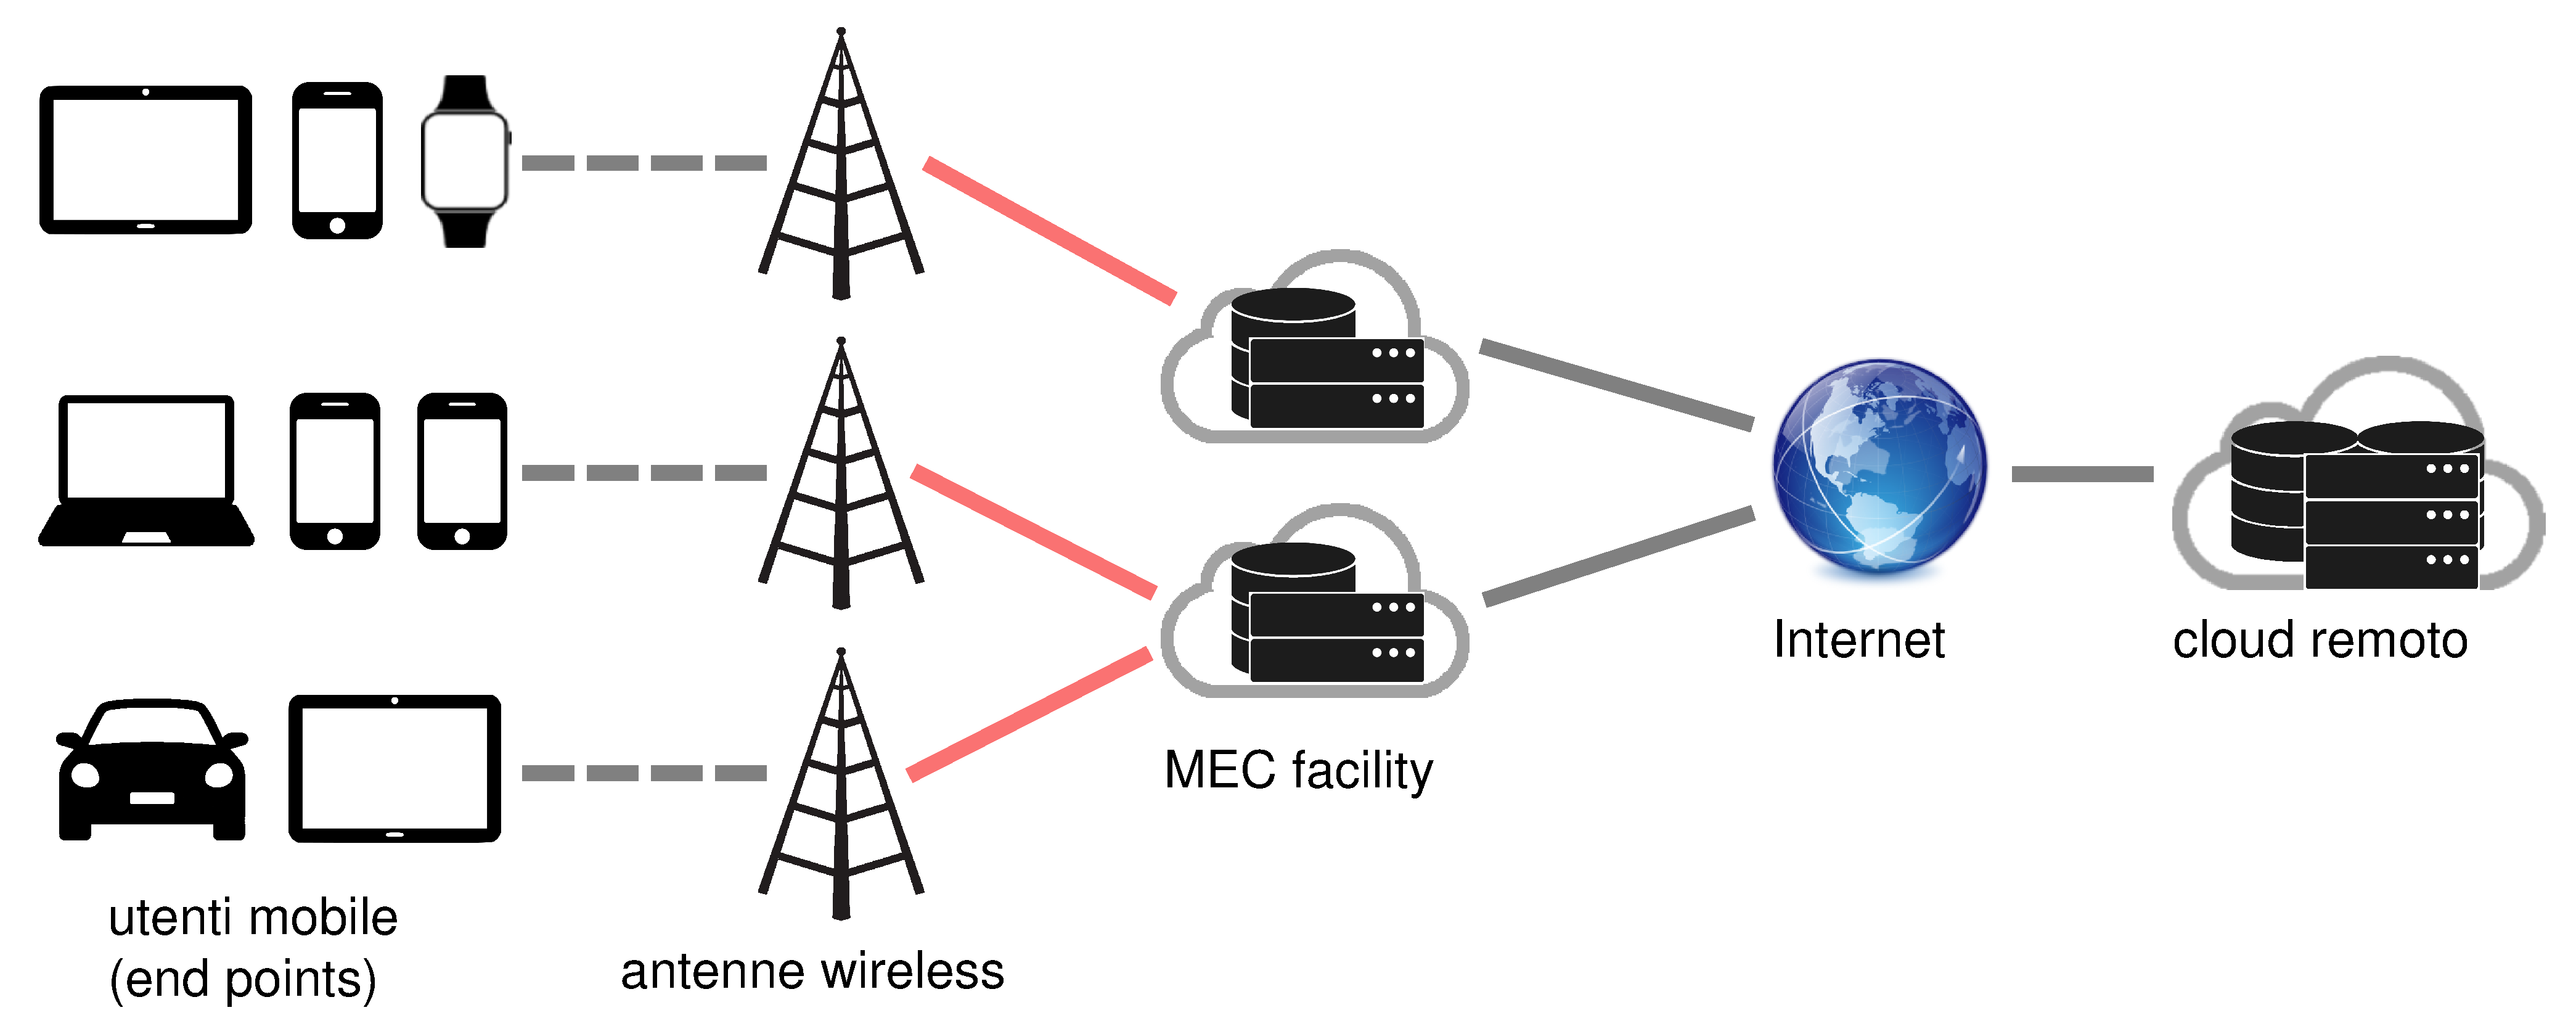
\includegraphics[width = 150mm]{img/esempio-infrastruttura-mec.pdf}
    \caption{Esempio di un'infrastruttura Mobile Edge Computing (MEC).}
    \label{fig:architettura-mec}
\end{figure}

Nella \hyperref[fig:architettura-mec]{figura 1} è presente un'infrastruttura MEC composta da due facility e tre AP, a cui sono collegati diversi dispositivi mobili di vario genere. Si noti come ogni dispositivo invii il proprio traffico all'AP a cui è collegato, e come tutto il traffico ricevuto da ciascuno sia inoltrato alla stessa facility. Si può osservare, per esempio, come all'AP nel mezzo siano connessi un laptop e due smartphone, mentre a quello in basso un'automobile smart ed un tablet. Nella figura, i due AP sono assegnati alla stessa facility (le linee rosse indicano gli assegnamenti) che riceverà e dovrà quindi gestire il traffico di tutti e cinque i dispositivi. Si noti infine come sia presente un cloud centralizzato che gestisce e sincronizza le varie facility della rete.


%
%   MODELLO DI ORCHESTRAZIONE
%
\section{Modello di orchestrazione proposto}
\label{sec:modello-di-orchestrazione-proposto}

Il modello di orchestrazione proposto rappresenta una variante di quello presentato negli articoli \cite{assignment-patterns} e \cite{analytics-mec}, in cui nell'effettuare le scelte di orchestrazione viene esplicitamente considerato l'utilizzo e la gestione dell'energia da parte dei siti edge.

Come illustrato in \cite{analytics-mec}, all'interno del modello viene introdotta una discretizzazione temporale che permette di effettuare migrazioni solo in determinati istanti, per esempio ogni 15 minuti. Questa scelta è ragionevole, dato che in caso contrario si pagherebbe un costo troppo elevato in termini di migrazione e spese generali dovute alla gestione del traffico. L'orizzonte temporale viene quindi rappresentato da un insieme di fascie temporali, chiamate anche `time-slot', della stessa durata.

L'obbiettivo del modello è quello di stabilire un piano degli assegnamenti che permetta di raggiungere un ragionevole compromesso tra: ottenere una buona qualità del servizio (cioè bassa latenza per l'utente finale), costi di migrazione contenuti e adeguata gestione energetica nelle facility. Nell'effettuare le scelte, bisogna tenere in considerazione che la domanda degli AP e l'energia prodotta varia nel corso del tempo, e inoltre che ogni facility possiede un limite massimo di domanda che è in grado di soddisfare simultaneamente. Si supponga inoltre che le batterie abbiano capacità limitata e che per gestire una unità di computazione sia necessaria una unità di energia.

\begin{figure}[t]
    \centering
    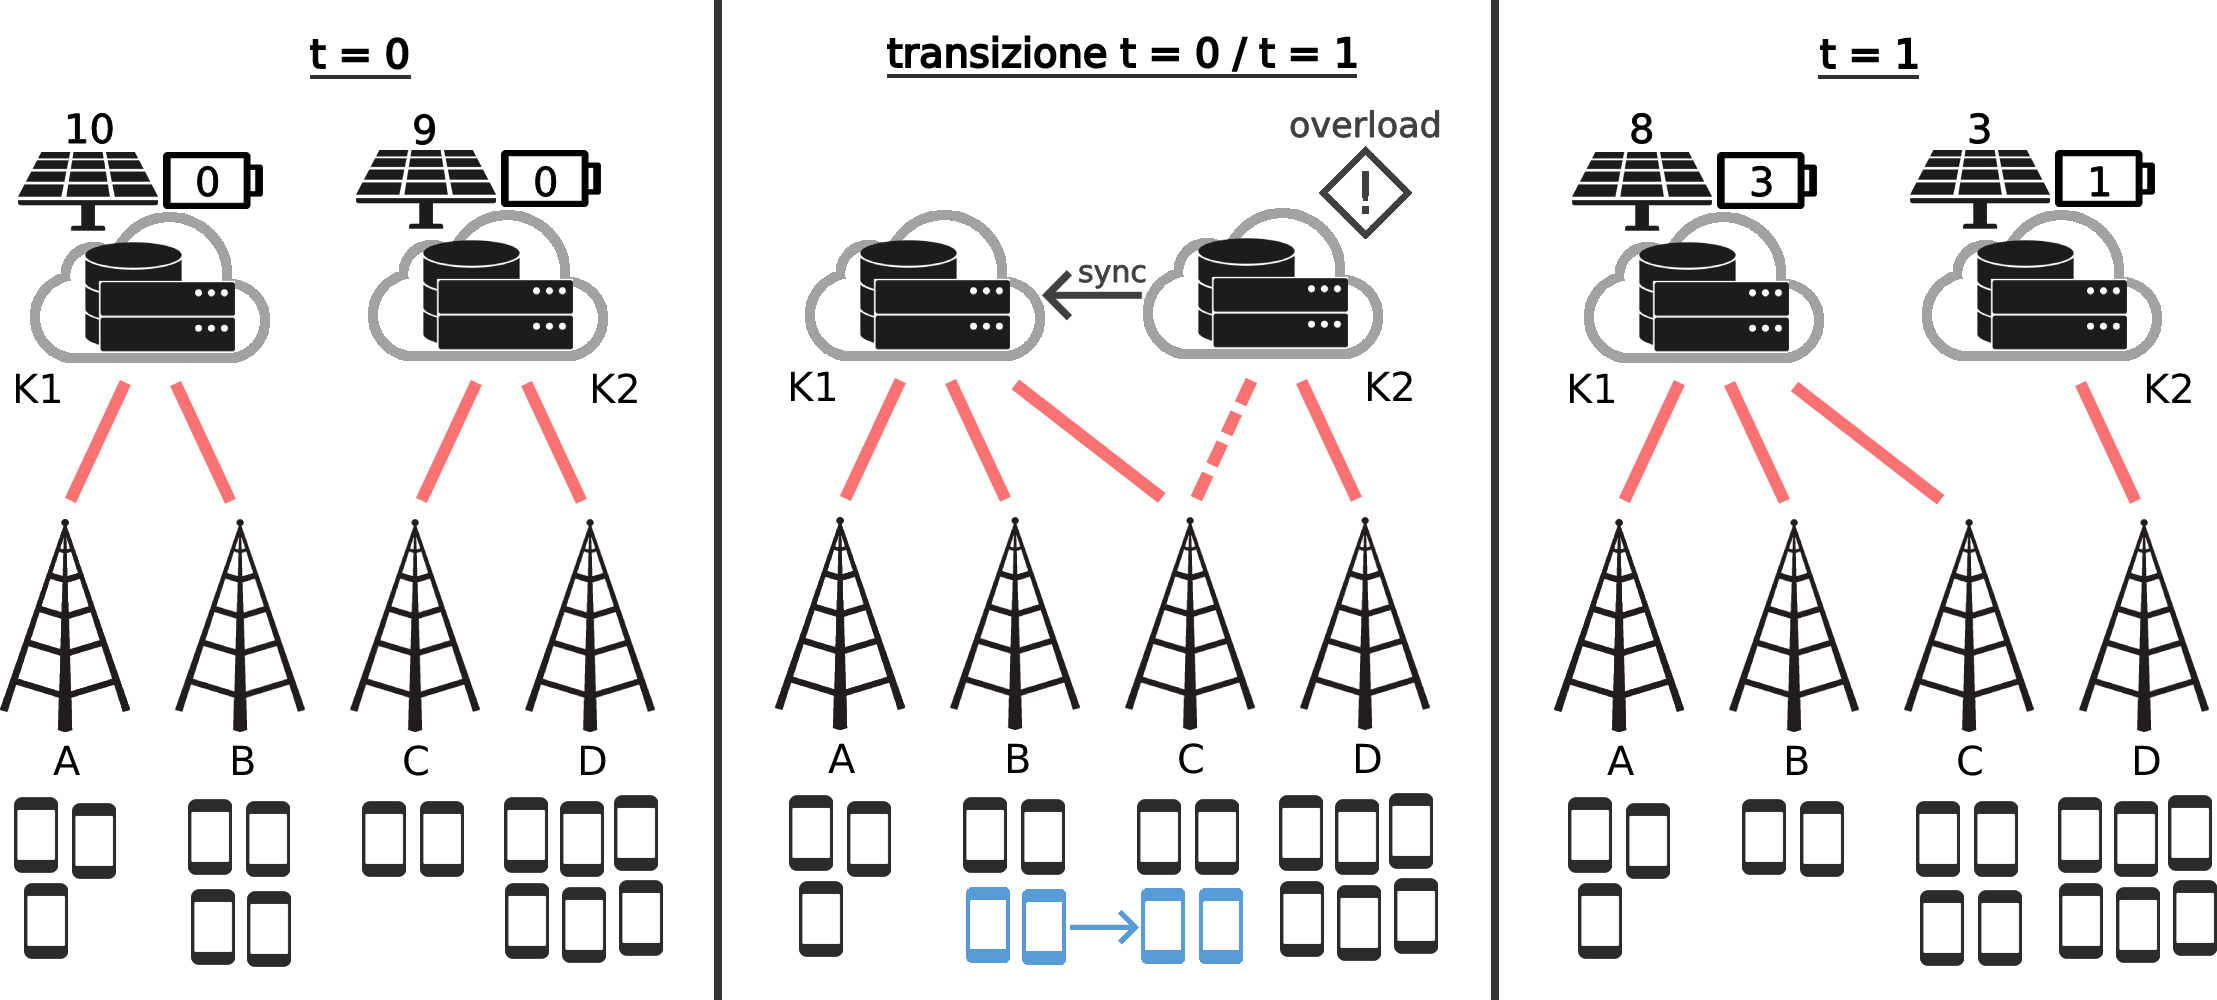
\includegraphics[width = 150mm]{img/esempio-assegnamenti.png}
    \caption{Esempio funzionamento del modello di orchestrazione.}
    \label{fig:esempio-assegnamenti}
\end{figure}


%
%   ESEMPIO FUNZIONAMENTO
%
\subsection{Esempio del funzionamento}
\label{sub-sec:esempio-funzionamento}

Una semplice applicazione di esempio è presentata nella \hyperref[fig:esempio-assegnamenti]{figura 2}. Come si può osservare, è presente una rete MEC con due facility (\texttt{K1} e \texttt{K2}) e quattro AP (\texttt{A}, \texttt{B}, \texttt{C}, \texttt{D}) considerata in due time-slot consecutivi (\texttt{t}=0, 1). Gli end point connessi agli AP sono rappresentati con dei piccoli rettangoli, e si supponga che inizialmente le batterie siano vuote in entrambe le facility. Nel primo time-slot (\texttt{t}=1) gli AP \texttt{A} e \texttt{B} sono associati alla facility \texttt{K1} mentre \texttt{C} e \texttt{D} a \texttt{K2}, quindi tutti gli utenti che sono connessi ad \texttt{A} e \texttt{B} avranno le proprie applicazioni in esecuzione su una VM presente in \texttt{K1}, mentre quelli connessi a \texttt{C} e \texttt{D} le avranno in \texttt{K2}. Questi assegnamenti permettono di avere una buona latenza, dato che ogni AP è connesso alla facility più vicina, ma anche una buona gestione energetica, in quanto nella facility \texttt{K1} vengono prodotte 10 unità di energia ed utilizzate solo 7, mentre in \texttt{K2} se ne producono 9 e utilizzano 8. In entrambi i casi avanzano delle unità (3 in \texttt{K1} e 1 in \texttt{K2}) che vengono immagazzinate nelle batterie per poter essere spese nel prossimo time-slot. Successivamente (transizione \texttt{t}=0/\texttt{t}=1) due utenti connessi all'AP \texttt{B} si spostano e si agganciano a \texttt{C}: a questo punto \texttt{K2} riceve una richiesta di domanda eccessiva che non riesce a gestire, e di conseguenza è necessario effettuare un'orchestrazione per ribilanciare il traffico. Questo comporta l'assegnare \texttt{C} a \texttt{K1}, ridimensionare le VM (aumentarne la potenza in \texttt{K1} e diminuirla in \texttt{K2}) e sincronizzare le facility, trasferendo lo stato delle VM riguardanti tutti gli utenti connessi a \texttt{C} da \texttt{K2} a \texttt{K1}. In un contesto reale, il modello deve prevenire una situazione di questo tipo, effettuando orchestrazioni preventive che tengano in considerazione la futura domanda dei vari AP, dato che questa circostanza va ad inficiare la qualità complessiva del servizio. Nel secondo time-slot (\texttt{t}=1) si avranno quindi gli AP \texttt{A}, \texttt{B} e \texttt{C} assegnati alla facility \texttt{K1}, mentre \texttt{D} a \texttt{K2}. Dal punto di vista energetico, la facility \texttt{K1} riesce a soddisfare la domanda di traffico (9 unità) utilizzando l'energia presente nella batteria e quella prodotta in questo time-slot (8 + 3 unità complessive). Per quanto riguarda invece \texttt{K2}, l'energia disponibile (3 + 1 unità) non è sufficiente, e quindi è necessario acquistare 2 ulterione unità. Da notare come l'energia potrebbe avere costi diversi nel corso dei time-slot, e di conseguenza potrebbe risultare conveniente acquistarla quando il costo è basso per immagazzinarla ed utilizzarla successivamente.


%
%   IMPLEMENTAZIONE
%
\subsection{Implementazione}
\label{sub-sec:implementazione}

Il comportamento del modello di orchestrazione fin qui descritto viene formulato secondo il formalismo della programmazione lineare misto-intera (MILP), ottenendo una variante del \textit{time-dependent generalized assignment problem} descritta nella \autoref{sec:modello-dinamico}. La prima opzione considerata è stata rivolvere direttamente il modello di programmazione matematica usando solver general purpose, in modo da determinare la soluzione ottima del problema, ma data la sua complettità, al crescere della dimensione dell'istanza, i tempi di calcolo aumentano fino a diventare proibitivi. Per questo motivo vengono successivamente proposti due algoritmi risolutivi eutistici, in modo da ottenere una risoluzione computazionalmente più efficiente. Nella \autoref{sec:semplificazione-modello} viene presentata la prima idea euristica, che mira ad abbassare la complessità semplificando il modello utilizzato, mentre nella \autoref{sec:aggregamento-time-slot} la seconda, che aggrega i time-slot dell'istanza per ottenerne una più facilmente risolvibile.
